%%%%%%%%%%%%%%%%%%%%%%%%%%%%%%%%%%%%%%%%%%%%%%%%%%%%%%%%%%%%%%%%%%%%%%%%%%%%%%%%
\chapter{Introduction}\label{ch:intro}
%%%%%%%%%%%%%%%%%%%%%%%%%%%%%%%%%%%%%%%%%%%%%%%%%%%%%%%%%%%%%%%%%%%%%%%%%%%%%%%%
The recovery of the underlying structure of a scene captured in an image is 
arguably one the core problems in Computer Vision. Although many properties
of a scene may be recovered, it is the geometry of the objects within the scene
that is of most use in many problems, as the geometry provides a strong model
from which to perform inference. In particular, the 3D shape of the underlying
objects is arguably the strongest cue for common tasks such as object
recognition and object localisation. However, the general problem or recovering
the 3D shape of an object from image (s) is incredibly ill-conditioned. Even when 
provided with multiple images, or additional information about the scene or
capturing conditions, 3D recovery is rife with ambiguities. As demonstrated
by~\cref{tbl:3d_recovery_methods}, many strategies have been proposed for
solving this problem. It is also important to note that they are two very
different outputs that can be obtained: \textit{dense shape
recovery} and \textit{sparse shape recovery.} Sparse shape recovery has been
well studied in areas such as Structure-from-Motion where it has been
employed for large-scale reconstruction of urban scenes~\cite{agarwal2009building,torr1998robust}.
However, dense shape recovery is a much more difficult problem as the necessary
complexity of the recovery problem increases. In this thesis I consider
only the problem of dense 3D shape recovery.

In contrast to the difficulty of the general case, the recovery of dense 3D
facial shape has been highly successful. Human faces have a number of qualities
that are highly desirable for shape recovery: they are extremely homogenous in
configuration (all healthy human faces have two eyes, a nose and mouth in the
same approximate location), convex, exhibit approximately lambertian 
reflectance~\cite{Sirovich:1987te,RefWorks:314,Basri:2003ie,RefWorks:98,Hallinan:1994dz},
are largely captured from a single direction (frontal) and are deformable
but not self occluding. Furthermore, there exists a large amount of publicly
available imagery of faces and human faces are of significant interest to a 
number of fields including entertainment, medicine and psychology.
%%%%%%%%%%%%%%%%%%%%%%%%%%%%%%%%%%%%%%%%
\begin{table}[t]
	\centering
	\resizebox{\textwidth}{!}{%
		\begin{tabular}{@{}llccl@{}}
		\toprule
		\multicolumn{1}{c}{Classification}                  & \multicolumn{1}{c}{Method}                                                   & \# Images & Other Input                                                                       & \multicolumn{1}{c}{Output} \\ \midrule
		\multirow{4}{*}[-0.7cm]{Image Formation}            & Shape-from-Shading                                                           & $1$       & \begin{tabular}[c]{@{}c@{}}Reflectance Model, \\ Lighting Directions\end{tabular} & Surface Normals            \\ \cmidrule(l){3-5} 
		                                                    & \begin{tabular}[c]{@{}l@{}} (Un) Calibrated \\ Photometric Stereo\end{tabular} & $\geq 3$  & \begin{tabular}[c]{@{}c@{}}Lighting Directions \\ (If Calibrated)\end{tabular}    & Surface Normals            \\ \cmidrule(l){3-5} 
		                                                    & Shape-from-Contour                                                           & $1$       & Object Contour                                                                    & Coarse Surface Normals     \\ \cmidrule(l){3-5} 
		                                                    & Analysis-by-Synthesis                                                        & $1$       & 3D Model                                                                          & 3D Shape                   \\ \midrule
		\multicolumn{1}{c}{\multirow{2}{*}{Photogrammetry}} & Multi-View Stereo                                                            & $k$       & Camera Extrinsics                                                                 & 3D Shape                   \\ \cmidrule(l){3-5} 
		\multicolumn{1}{c}{}                                & Structure-from-Motion                                                        & $k$       & Corresponding Points                                                              & 3D Shape                   \\ \midrule
		\multicolumn{1}{c}{Other}                           & Shape Transfer                                                               & $1$       & 3D Model                                                                          & 3D or 2.5D Shape           \\ \bottomrule
		\end{tabular}
	}
	\caption{A summary of methods for recovering 3D shape from images. The two 
	         largest subcategories are image formation algorithms and 
	         photogrammetry.}
\label{tbl:3d_recovery_methods}
\end{table}
%%%%%%%%%%%%%%%%%%%%%%%%%%%%%%%%%%%%%%%%
An impressive example of the quality of 3D reconstruction possible is the
seminal work of Blanz and Vetter~\cite{RefWorks:96}. A commercial example of the
quality of reconstruction provided by a 3D Morphable Model (3DMM) method
is given in~\cref{fig:facegen_tom_hanks}. However, despite the success of 
3DMMs~\cite{RefWorks:96}, the problem of high quality 3D facial 
surface recovery from challenging images is still far from solved. For example,
the recovery of 3D facial surfaces under arbitrary conditions,
so called ``in-the-wild'' images, remains a challenging and active area of
research~\cite{KemelmacherShlizerman:2013iv,Suwajanakorn:2015gf,Suwajanakorn:2014bl,Snape:2015gl,Roth:2015hq}.
In the case of 3DMMs, ``in-the-wild'' images present a significant challenge
as 3DMMs attempt to recover shape via an ``analysis-by-synthesis'' approach. An
``analysis-by-synthesis'' approach involves attempting to minimise the 
reconstruction error between the input image and a rendered output image that
is modelled via a set of parametric models and lighting conditions. Therefore,
in the case of ``in-the-wild'' facial images, ``analysis-by-synthesis'' is
incredibly challenging as an accurate result would require photorealistic
rendering, which is currently not possible within the Computer Vision
literature. Moreover, the parametric models employed contain a low number
of parameters and therefore have a tendency of being smooth and thus are not 
able to model fine details such as wrinkles.

Due to the insufficiencies of generic shape recovery, it is common to assume
that aspects of the scene are known apriory. In the case of the 3DMM, it is 
assumed that we know the class of object e.g faces and that we know the
approximate location of the face in the image. Knowing the class of object is
a strong but very powerful prior. This is most commonly exploited by introducing
some form of template or parametric model that describes the shape space of the
object class in question. However, there is a crucial problem that must be
solved before these shape priors can be employed. This is the problem of
\textit{correspondance}. For example, the 3DMM algorithm treats the entire
shape recovery problem as a correspondance problem in which the 3D shape
model is used to synthesize an image which is then aligned in image space
with the input image. Another example is the seemingly unrelated area of 
Structure-from-Motion, whereby a set of correspondances amongst a number
of images is assumed. These corresponding points are then factorized in order
to recover both the underlying 3D shape and the parameters of the camera 
projection matrices that produced the input 2D points. In this case, the 
correspondance problem is assumed to have been already solved. Therefore,
when considering 3D facial shape recovery methods it is also important
to consider the problem of correspondance.
%%%%%%%%%%%%%%%%%%%%%%%%%%%%%%%%%%%%%%%%
\begin{figure}[t]
	\centering
	\hspace*{\fill}
	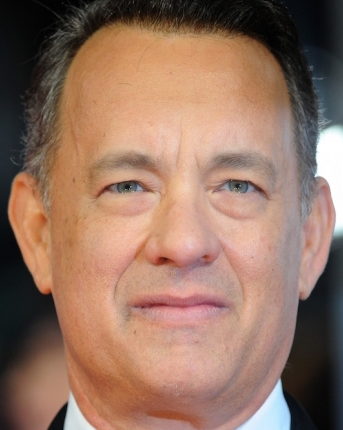
\includegraphics[height=1.8in]{introduction/images/tom_hanks_frontal_awards}\hfill
	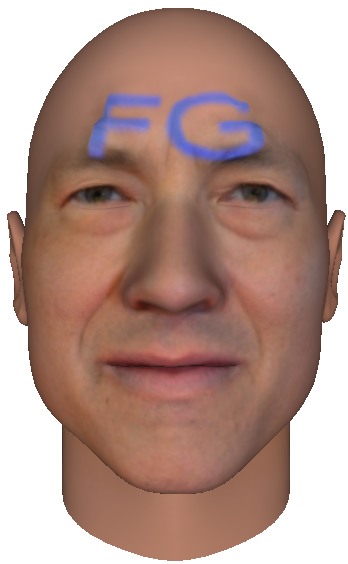
\includegraphics[height=1.8in]{introduction/images/tom_hanks_frontal_awards_facegen}\hfill
	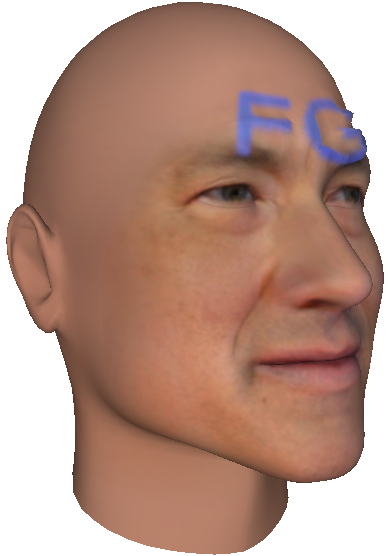
\includegraphics[height=1.8in]{introduction/images/tom_hanks_frontal_awards_facegen_profile}\hfill
	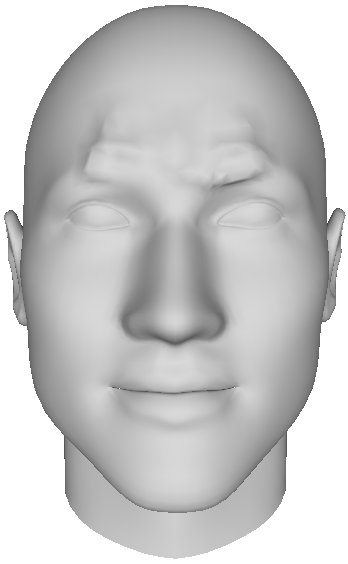
\includegraphics[height=1.8in]{introduction/images/tom_hanks_frontal_awards_facegen_no_texture}\hfill
	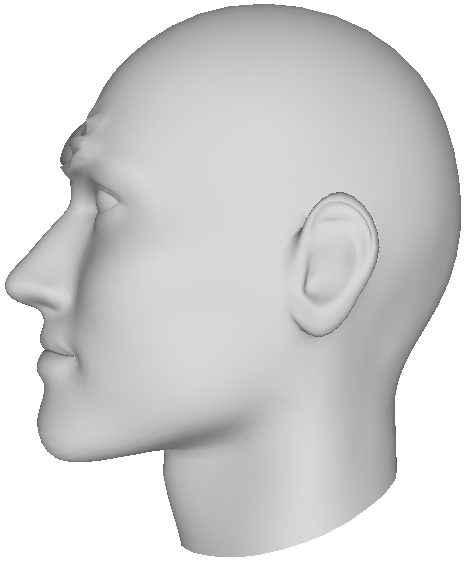
\includegraphics[height=1.8in]{introduction/images/tom_hanks_frontal_awards_facegen_no_texture_profile}
	\hspace*{\fill}
	\caption{An example of facial shape recovery by a 3D Morphable Model, 
	         provided by the commercial FaceGen software~\cite{facegen}. The
	         input image (leftmost) of Tom Hanks was provided and keypoints were
	         manually specified. Notice that the texture provides a strong 
	         likeness to Tom Hanks' face, yet the untextured mesh does not.}
\label{fig:facegen_tom_hanks}
\end{figure}
%%%%%%%%%%%%%%%%%%%%%%%%%%%%%%%%%%%%%%%%

In this thesis, I am interested in tackling the problem of 3D facial shape
recovery from challenging ``in-the-wild'' conditions. This is in contrast
to many works, such as the 3DMM, that focus on the recovery of facial shape
under ideal conditions (uniform frontal illumination, frontal face,
no expression, young caucasian subject). As previously mentioned and summarised
in \cref{tbl:3d_recovery_methods}, there are 
a number of scenarios that may be considered in order to recover shape from
images. Given the breadth of possible scenarios, I have categorised them into
three major areas:
%%%%%%%%%%%%%%%%%%%%%%%%%%%%%%%%%%%%%%%%
\begin{itemize}
	\item \textbf{Single Image.} Given a single image, estimate the facial 
	      shape. This may involve employing template facial shapes, parametric
	      facial models or knowledge of the lighting conditions. 
	\item \textbf{Image Collections.} Given multiple images of faces, that may
	      or may not be of the same individual, estimate the facial shape for
	      each image. This may involve parametric models, employing illumination
	      constraints or known correspondances between the images.
	\item \textbf{Videos.} Given a sequence of images of a single individual,
	      recover their facial shape. This may involve known correspondances or
	      parametric models.
\end{itemize}
%%%%%%%%%%%%%%%%%%%%%%%%%%%%%%%%%%%%%%%%
Although there exists many more scenarios than those just described, 
these three provide methods of recovery for the vast majority of media 
available for faces. In this thesis, I chose to investigate a novel method
for improving the state-of-the-art under each of these three scenarios. The rest
of this section will be devoted to describing my contributions in the area 
of dense 3D facial shape recovery.
%%%%%%%%%%%%%%%%%%%%%%%%%%%%%%%%%%%%%%%%%%%%%%%%%%%%%%%%%%%%%%%%%%%%%%%%%%%%%%%%
\section{Contributions}\label{sec:intro_contrib}
%%%%%%%%%%%%%%%%%%%%%%%%%%%%%%%%%%%%%%%%%%%%%%%%%%%%%%%%%%%%%%%%%%%%%%%%%%%%%%%%

%%%%%%%%%%%%%%%%%%%%%%%%%%%%%%%%%%%%%%%%%%%%%%%%%%%%%%%%%%%%%%%%%%%%%%%%%%%%%%%%
\section{Publications}\label{sec:intro_pubs}
%%%%%%%%%%%%%%%%%%%%%%%%%%%%%%%%%%%%%%%%%%%%%%%%%%%%%%%%%%%%%%%%%%%%%%%%%%%%%%%%
In this section I provide a list of publication that were authored during the
course of my thesis. These publications are split into two sections, those
that are related to the contents of this thesis 
(\cref{subsec:intro_rel_pubs}) and other publications that 
are not directly relevant (\cref{subsec:intro_other_pubs}).
%%%%%%%%%%%%%%%%%%%%%%%%%%%%%%%%%%%%%%%%%%%%%%%%%%%%%%%%%%%%%%%%%%%%%%%%%%%%%%%%
\subsection{Related Publications}\label{subsec:intro_rel_pubs}
%%%%%%%%%%%%%%%%%%%%%%%%%%%%%%%%%%%%%%%%%%%%%%%%%%%%%%%%%%%%%%%%%%%%%%%%%%%%%%%%
%%%%%%%%%%%%%%%%%%%%%%%%%%%%%%%%%%%%%%%%
\begin{itemize}
	\item\bibentry{Snape:2014de}
	\item\bibentry{Snape:2015gl}
	\item\bibentry{Snape:2015hj}
\end{itemize}
%%%%%%%%%%%%%%%%%%%%%%%%%%%%%%%%%%%%%%%%
%%%%%%%%%%%%%%%%%%%%%%%%%%%%%%%%%%%%%%%%%%%%%%%%%%%%%%%%%%%%%%%%%%%%%%%%%%%%%%%%
\subsection{Other Publications}\label{subsec:intro_other_pubs}
%%%%%%%%%%%%%%%%%%%%%%%%%%%%%%%%%%%%%%%%%%%%%%%%%%%%%%%%%%%%%%%%%%%%%%%%%%%%%%%%
%%%%%%%%%%%%%%%%%%%%%%%%%%%%%%%%%%%%%%%%
\begin{itemize}
	\item\bibentry{menpo14}
	\item\bibentry{Chrysos:2015gt}
\end{itemize}
%%%%%%%%%%%%%%%%%%%%%%%%%%%%%%%%%%%%%%%%
The publications above are the joint work of the authors listed and do not
contain significant contributions to this thesis. Unless explicitly stated,
these publications are not considered to be my sole work.
%%%%%%%%%%%%%%%%%%%%%%%%%%%%%%%%%%%%%%%%%%%%%%%%%%%%%%%%%%%%%%%%%%%%%%%%%%%%%%%%
\section{Outline}\label{sec:introduction_outline}
%%%%%%%%%%%%%%%%%%%%%%%%%%%%%%%%%%%%%%%%%%%%%%%%%%%%%%%%%%%%%%%%%%%%%%%%%%%%%%%%
\cref{ch:background} provides a thorough literature review of existing
methodologies for 3D facial shape recovery. This includes relevant literature
for sparse and dense shape recovery, in order to provide a complete
picture as to the current state-of-the-art in 3D facial shape recovery.
\cref{ch:singl_imag} introduces my contribution in the area of single image
facial shape recovery. A kernel method for representing surface normals is 
introduced and this kernel is used in a number of areas including 2D and 3D
image alignment and Shape-from-Shading.
\cref{ch:imag_coll} proposes a explicit algorithmic formulation for recovering
surface normals from unconstrained collections of facial images. This method,
dubbed Class-Specific Photometric Stereo, extends existing work on Uncalibrated
Photometric Stereo~\cite{KemelmacherShlizerman:2013iv,basri2007photometric}
with a robust method of recovering a per-image spherical harmonics.
\cref{ch:face_flow} considers the problem of dense facial correspondances. By
treating facial correspondance as a 2D image alignment problem, dense
correspondances between a parametric facial model and an image sequence are
computed. This model is easily extended to recover a 3D surface by leveraging
the correspondances between the image and a 3D model. 
Finally, \cref{ch:conclusions} summarises the findings of the previous chapters
and introduces possible areas of further research. 
%%%%%%%%%%%%%%%%%%%%%%%%%%%%%%%%%%%%%%%%%%%%%%%%%%%%%%%%%%%%%%%%%%%%%%%%%%%%%%%%